% -*- root: projekt.tex -*-

%\chapter{Obsah CD}
%\chapter{Manual}
%\chapter{Konfigrační soubor}
%\chapter{RelaxNG Schéma konfiguračního soboru}
%\chapter{Plakat}

\newcommand\cmdarglist[1]{
    \begin{description}#1\end{description}
}

\newcommand\cmdarg[2]{
    \item[\texttt{#1}] \hfill \\
    #2
}

\newcommand\cmdargdef[3]{
    \item[\texttt{#1}] (výchozí: #2) \hfill \\
    #3
}

\chapter{Uživatelská příručka}
\label{apxManual}

\section{Překlad programu}

Program je rozdělen do několika modulů. Jejich překlad a sestavení výsledného programu je definován v~Makefile a spouští se příkazem \texttt{make}. Je potřeba překladač GCC ve verzi alespoň 4.8, lépe ve verzi 4.9, která má dokonalejší podporu SIMD instrukcí, zejména umí využít všechny dostupné registry. Kvůli některým použitým funkcím (např. pro získání spotřebovaného procesorového času) musí operační systém implementovat standard POSIX. Program byl testován na systémech Ubuntu 12.04 a na superpočítači Anselm, který používá systém bullx Linux odvozený od Red Hat Enterprise Linux.

Pokud překlad končí chybou a na výstupu jsou takovéto zprávy:

\begin{lstlisting}[language=]
/tmp/ccQ9hvQS.s: Assembler messages:
/tmp/ccQ9hvQS.s:33: Error: suffix or operands invalid for `vpcmpeqd'
/tmp/ccQ9hvQS.s:85: Error: suffix or operands invalid for `vpcmpeqd'
/tmp/ccQ9hvQS.s:92: Error: suffix or operands invalid for `vpcmpeqd'
\end{lstlisting}

\noindent{}je třeba z Makefile odstranit z proměnné \texttt{CFLAGS} část \texttt{-DAVX2}, čímž se vypne kompilace kódu akcelerovaného pomocí instrukcí AVX2. Chyby jsou s největší pravděpodobností způsobeny tím, že použitý překladač je novější verze a generuje kód, kterému použitý assembler nerozumí\footnote{Zdroj: \url{http://code.compeng.uni-frankfurt.de/issues/718}}. Tento problém se vyskytl na Anselmu, který AVX2 nepodporuje.

Jednotlivé moduly programu se překládají samostatně do složky \texttt{build}. Při změnách ve zdrojovém kódu tak není nutné opakovaně překládat moduly, do kterých se nezasahovalo. Výstupem překladu je několik spustitelných souborů:

\begin{itemize}
    \item \texttt{coco}\footnote{Název \texttt{coco} je zkratka pro COlearning in COevolution.} -- hlavní program, samotný evoluční návrh obrazových filtrů,
    \item \texttt{coco\_apply} -- aplikace filtru uloženého v~souboru \texttt{*.chr} na libovolný obrázek,
    \item \texttt{coco\_predvis} -- vizualizace použitých prediktorů fitness,
    \item \texttt{coco\_predhist} -- tvorba histogramu pixelů používaných v~prediktorech fitness.
\end{itemize}

\section{Formáty souborů}

\subsubsection*{Obrázky}

Načítání trénovacích obrázků je řešeno pomocí knihovny \texttt{stb\_image.h}\footnote{\url{https://github.com/nothings/stb}}. Jsou tedy podporovány formáty implementované v~této knihovně, s~většími či menšími omezeními: JPEG, PNG, TGA, BMP, PSD, GIF, HRD, PIC. Všechny obrázky musí být uloženy ve stupních šedi, 8 bitů na pixel. Testovány byly pouze obrázky ve formátech BMP a PNG. Výstupní obrázky (např. výstup nejlepšího filtru) jsou ukládány vždy ve formátu PNG.

\subsubsection*{Obrazové filtry}

Chromozomy obrazových filtrů jsou ukládány do textového formátu, který je totožný s~formátem, který používá program CGP Viewer od Zdeňka Vašíčka, který vypadá takto:

\begin{lstlisting}
{2, 2, 4, 1, 2, 1, 16}                                  %*\Comment{Konfigurace CGP}*
([3] 0, 1, 2)([4] 2, 1, 2)([5] 0, 2, 13)([6] 3, 4, 6)   %*\Comment{Vstupy a funkce bloků}*
(5, 4)                                                  %*\Comment{Primární výstupy}*
\end{lstlisting}

Na začátku je ve složených závorkách uvedena konfigurace mřížky a funkčních bloků: počet primárních vstupů, primárních výstupů, šířka a výška mřížky, počet vstupů a výstupů funkčních bloků a počet možných funkcí, které může blok vykonávat. Dále jsou pro každý blok v~kulatých závorkách uvedeny jeho číslo (v~hranatých závorkách) a jeho geny: čísla bloků, na které jsou připojené jeho vstupy a číslo funkce, kterou vykonává. Na závěr jsou v~kulatých závorkách uvedeny čísla bloků, kam jsou připojeny primární výstupy programu.

Kromě tohoto formátu jsou filtry ukládány také jako kód v~jazyce C a v~textovém formátu srozumitelném pro uživatele, který pro stejný program vypadá takto:

{
    \centering
    \vskip\baselineskip
    \begin{BVerbatim}[fontsize=\footnotesize]
         .------------------------------------------------------------------------.
         |      .----.            .----.            .----.            .----.      |
    [ 0]>| [ 0]>|    |>[ 2]  [ 2]>|    |>[ 3]  [ 0]>|    |>[ 4]  [ 3]>|    |>[ 5] |>[5]
    [ 1]>| [ 1]>| f2 |       [ 1]>| f2 |       [ 2]>| f13|       [ 4]>| f6 |      |>[4]
         |      '----'            '----'            '----'            '----'      |
         '------------------------------------------------------------------------'
    \end{BVerbatim}
}

\section{Spuštění evoluce obrazových filtrů}

Povinné parametry jsou pouze dva, a sice:

\begin{itemize}
    \item \texttt{-{}-noisy FILE} nebo \texttt{-n FILE}
    \item \texttt{-{}-original FILE} nebo \texttt{-i FILE}
\end{itemize}

Jména souborů se zdrojovým (poškozeným) a cílovým (nepoškozeným) obrázkem. V~případě detekce hran se u~parametru \texttt{-{}-noisy} uvede zdrojový obrázek a u~\texttt{-{}-original} obrázek s~vyznačenými hranami.

Ostatní parametry jsou volitelné, pokud nejsou uvedeny, použije se výchozí hodnota.

\subsection*{Parametry evoluce}

\cmdarglist{
    \cmdargdef{-{}-algorithm ALG, -a ALG}{\texttt{coev}}{
        Algoritmus evoluce:
        \begin{itemize}
            \item \texttt{cgp} -- standardní CGP,
            \item \texttt{coev} -- koevoluce s~pevnými prediktory fitness,
            \item \texttt{colearn} -- koevoluce se souběžným učením.
        \end{itemize}
    }

    \cmdargdef{-{}-random-seed N, -r N}{dle \texttt{gettimeofday()}}{
        Inicializační hodnota generátoru pseudonáhodných čísel.
    }

    \cmdarg{-{}-target-psnr N, -t N}{
        Evoluce se ukončí po dosažení zvolené hodnoty PSNR.
    }

    \cmdarg{-{}-target-fitness N, -f N}{
        Evoluce se ukončí po dosažení zvolené fitness. Jde o~hodnotu zlomku ve výpočtu PSNR, jak je uvedeno v části~\ref{secImplFitness}.
    }
}

\subsection*{Parametry sběru dat}

\cmdarglist{
    \cmdarg{-{}-log-dir DIR, -l DIR}{
        Složka, do které se uloží záznamy o~běhu. Pokud neexistuje, bude vytvořena. Její obsah popisuje sekce \ref{apxManualLogDir}.
    }

    \cmdarg{-{}-log-interval N, -k N}{
        Kromě záznamů při změně fitness filtru, zapíše do logu také každou N-tou generaci.
    }

    \cmdarg{-{}-log-pred-file FILE}{
        Do souboru \texttt{FILE} zapíše obsah všech prediktorů použitých při ohodnocování fitness. Soubor lze dále zpracovat nástroji \texttt{coco\_predhist} a \texttt{coco\_predvis}.
    }
}

\subsection*{Parametry populace obrazových filtrů}

\cmdarglist{
    \cmdargdef{-{}-cgp-mutate N, -m N}{5}{
        Maximální počet pozměněných genů filtru při mutaci.
    }

    \cmdargdef{-{}-cgp-population-size N, -p N}{8}{
        Počet jedinců v~populaci filtrů.
    }

    \cmdargdef{-{}-cgp-archive-size N, -s N}{8}{
        Velikost archivu filtrů pro ohodnocování prediktorů.
    }
}

\subsection*{Parametry populace prediktorů fitness}

\cmdarglist{
    \cmdargdef{-{}-pred-size N, -S N}{0,25}{
        Velikost genotypu prediktorů v~procentech (jako desetinné číslo). V~případě souběžného učení je vhodné uvést hodnotu 1.
    }

    \cmdargdef{-{}-pred-mutate N, -M N}{5}{
        Maximální procento pozměněných genů prediktoru při mutaci.
    }

    \cmdargdef{-{}-pred-population-size N, -P N}{32}{
        Počet jedinců v~populaci prediktorů.
    }

    \cmdargdef{-{}-pred-type TYPE, -T TYPE}{\texttt{permuted} nebo \texttt{repeated} dle \texttt{-{}-algorithm}}{
        Typ prediktoru:
        \begin{itemize}
            \item \texttt{permuted} -- genotyp bez duplicitních genů, výchozí pro koevoluci s~fixními prediktory (\texttt{-a coev}), nelze použít při souběžném učení,
            \item \texttt{repeated} -- s~duplicitními geny, výchozí pro souběžné učení (\texttt{-a colearn}),
            \item \texttt{repeated-circular} -- s~duplicitními geny, offset tvorby fenotypu se určí jako nejlepší z~5 náhodných možností.
        \end{itemize}
    }
}

\subsection*{Parametry souběžného učení}

\cmdarglist{
    \cmdargdef{-{}-bw-pred-initial-size N, -I N}{hodnota \texttt{-{}-pred-size}}{
        Počáteční velikost prediktoru (hodnota \emph{UsedGenes)} v procentech. Nesmí být vyšší než celková velikost prediktoru (daná parametrem \texttt{-{}-pred-size}).
    }

    \cmdargdef{-{}-bw-pred-min N, -N N}{0}{
        Minimální velikost prediktoru (hodnota \emph{UsedGenes}) v procentech.
    }

    \cmdargdef{-{}-baldwin-interval NUM, -b NUM}{0}{
        Maximální počet generací CGP mezi dvěma změnami velikost prediktoru. Hodnota 0 znamená, že se velikost upravuje jen při změně rodiče v populaci filtrů.
    }

    \cmdargdef{-{}-bw-inac-tol N}{1,2}{Parametr $I_\mathit{threshold}$}
    \cmdargdef{-{}-bw-inac-coef N}{2}{Parametr $c_I$}
    \cmdargdef{-{}-bw-zero-eps N}{0,001}{Parametr $v_\mathit{zero}$}
    \cmdargdef{-{}-bw-slow-thr N}{0,1}{Parametr $v_\mathit{slow}$}

    \cmdarg{-{}-bw-by-max-length}{
        Změna velikost prediktoru je vypočtena z celkového počtu případů fitness a ne relativně k současné velikosti. Při použití této volby se namísto parametrů \texttt{-{}-bw-XXXX-coef} používají parametry \texttt{-{}-bw-XXXX-inc}
    }

    \cmdargdef{-{}-bw-zero-coef N}{0,9}{Parametr $c_{0}$ (pokud není použito \texttt{-{}-bw-by-max-length})}
    \cmdargdef{-{}-bw-decr-coef N}{0,96}{Parametr $c_{-1}$ (pokud není použito \texttt{-{}-bw-by-max-length})}
    \cmdargdef{-{}-bw-slow-coef N}{1,07}{Parametr $c_{+1}$ (pokud není použito \texttt{-{}-bw-by-max-length})}
    \cmdargdef{-{}-bw-fast-coef N}{1}{Parametr $c_{+2}$ (pokud není použito \texttt{-{}-bw-by-max-length})}

    \cmdargdef{-{}-bw-zero-inc N}{-0,01}{Parametr $c_{0}$ (při použití \texttt{-{}-bw-by-max-length})}
    \cmdargdef{-{}-bw-decr-inc N}{-0,07}{Parametr $c_{-1}$ (při použití \texttt{-{}-bw-by-max-length})}
    \cmdargdef{-{}-bw-slow-inc N}{0,01}{Parametr $c_{+1}$ (při použití \texttt{-{}-bw-by-max-length})}
    \cmdargdef{-{}-bw-fast-inc N}{0}{Parametr $c_{+2}$ (při použití \texttt{-{}-bw-by-max-length})}
}

%\section{Výstupy programu}

\section{Nástroj coco\_apply}

Tento nástroj slouží pro aplikaci evolvovaného filtru na libovolný obrázek, volitelně i pro výpočet PSNR a vizualizace zapojení filtru.

\subsection*{Povinné parametry}

\cmdarglist{
    \cmdarg{-{}-chromosome FILE, -c FILE}{
        Soubor s uloženým chromozomem filtru ve formátu pro CGP Viewer.
    }
    \cmdarg{-{}-input FILE, -i FILE}{
        Vstupní obrázek filtru. Pokud není uveden nebo se uvede \texttt{-}, použije se standardní vstup.
    }
    \cmdarg{-{}-output FILE, -o FILE}{
        Výstupní obrázek filtru. Pokud není uveden nebo se uvede \texttt{-}, použije se standardní výstup.
    }
}

\subsection*{Volitelné parametry}

\cmdarglist{
    \cmdarg{-{}-calc-psnr REFIMG, -p REFIMG}{
        Na chybový výstup vypíše PSNR výstupního obrázku a referenčního obrázku.
    }
    \cmdarg{-{}-print-ascii, -a}{
        Na chybový výstup vypíše zapojení filtru ve formě ASCII Artu.
    }
    \cmdarg{-{}-output FILE, -o FILE}{
        Výstupní obrázek filtru.
    }
}

\section{Nástroj coco\_predhist}

Tento nástroj slouží pro tvorbu histogramů vybíraných prediktorů. Na standardní výstup vypíše počet použití každého devítiokolí ve formátu CSV. Volitelně vytvoří i 2D histogram jako obrázek.

\subsection*{Povinné parametry}

\cmdarglist{
    \cmdarg{-{}-width X, -x X}{
        Šířka obrázku používaného při evoluci.
    }
    \cmdarg{-{}-height Y, -y Y}{
        Výška obrázku používaného při evoluci.
    }
    \cmdarg{-{}-generations N, -g N}{
        Počet generací, pro které se vytvoří histogram.
    }
    \cmdarg{LOGFILE}{
        Za přepínači se uvedou jména jednoho či více souborů s výpisem použitých prediktorů, který se vygeneruje při evoluci pomocí parametru \texttt{-{}-log-pred-file}.
    }
}

\subsection*{Volitelné parametry}

\cmdarglist{
    \cmdarg{-{}-output-image FILE, -o FILE}{
        Vytvoří 2D histogram a uloží jej jako obrázek PNG do souboru \texttt{FILE}.
    }
}

\section{Nástroj coco\_predvis}

Tento nástroj slouží pro tvorbu vizualizaci všech použitých prediktorů. Na standardní výstup vypíše číslo generace a počet obsažených devítiokolí pro každý použitý prediktor. Volitelně vizualizuje použité pixely v každém prediktoru. Takto byly vygenerovány histogramy na obrázku \ref{obrPredhist}.

\subsection*{Povinné parametry}

\cmdarglist{
    \cmdarg{-{}-log FILE, -l FILE}{
        Soubor s výpisem použitých prediktorů, který se vygeneruje při evoluci pomocí parametru \texttt{-{}-log-pred-file}.
    }
}

\subsection*{Povinné parametry pro vizualizaci}

\cmdarglist{
    \cmdarg{-{}-image FILE, -i FILE}{
        Podkladový obrázek pro vizualizaci prediktorů. Typicky jde o obrázek používaný při evoluci.
    }
    \cmdarg{-{}-outdir FILE, -o FILE}{
        Složka, do které se uloží vizualizované prediktory. Soubory jsou pojmenovávány podle čísla generace. Pokud složka neexistuje, vytvoří se.
    }
}

\subsection*{Volitelné parametry pro vizualizaci}

\cmdarglist{
    \cmdargdef{-{}-color RRGGBB, -o RRGGBB}{červená (\texttt{FF0000})}{
        Barva bodů, které při vizualizaci označují použitá devítiokolí. Zadává se v hexadecimálním \uv{HTML} formátu.
    }
}

\chapter{Výsledky experimentů}
\label{apxResults}

Následující grafy zobrazují kvalitu získaných filtrů pomocí standardního CGP, koevoluce prediktorů fitness různé velikosti a koevoluce se souběžným učením (sloupce \uv{R} pro $\mathit{FP_{REL}}$ a \uv{A} pro $\mathit{FP_{ABS}}$). Hodnota PSNR je průměr pro 12 testovacích obrázků (viz obrázek~\ref{obrTestovaci}). Čas běhu programu je určen jako součet procesorového času všech vláken. Pro každou intenzitu šumu (resp. pro detektor hran) a pro každý algoritmus a nastavení bylo provedeno 100 nezávislých běhů.

\section{Šum typu sůl a pepř}

\begin{figure}[H]
    \centering
    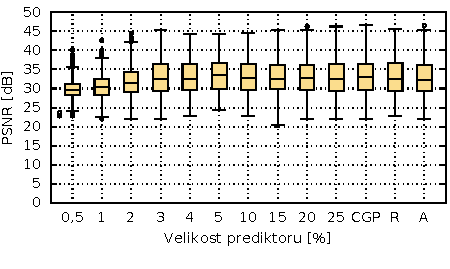
\includegraphics[width=0.475\textwidth]{fig/plot/compare/saltpepper5-100kg-psnrtest.pdf}
    \hskip0.5cm
    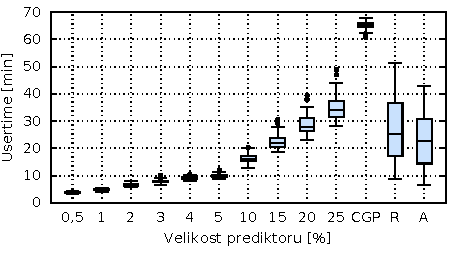
\includegraphics[width=0.475\textwidth]{fig/plot/compare/saltpepper5-100kg-usertime.pdf}
    \caption{5\% šum typu sůl a pepř}
\end{figure}

\begin{figure}[H]
    \centering
    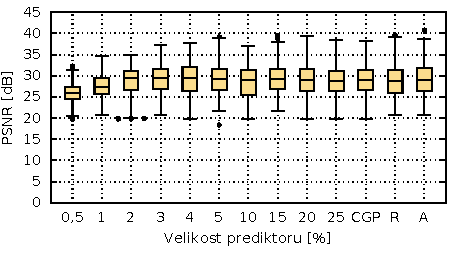
\includegraphics[width=0.475\textwidth]{fig/plot/compare/saltpepper10-100kg-psnrtest.pdf}
    \hskip0.5cm
    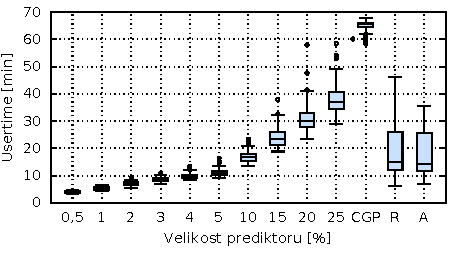
\includegraphics[width=0.475\textwidth]{fig/plot/compare/saltpepper10-100kg-usertime.pdf}
    \caption{10\% šum typu sůl a pepř}
\end{figure}

%\clearpage

\begin{figure}[H]
    \centering
    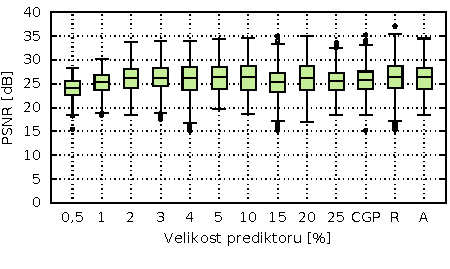
\includegraphics[width=0.475\textwidth]{fig/plot/compare/saltpepper15-100kg-psnrtest.pdf}
    \hskip0.5cm
    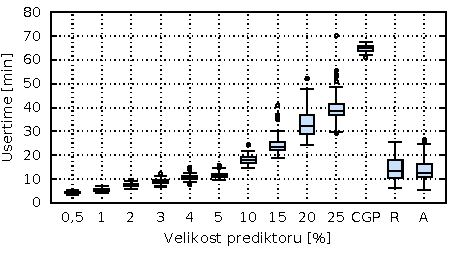
\includegraphics[width=0.475\textwidth]{fig/plot/compare/saltpepper15-100kg-usertime.pdf}
    \caption{15\% šum typu sůl a pepř}
\end{figure}

\begin{figure}[H]
    \centering
    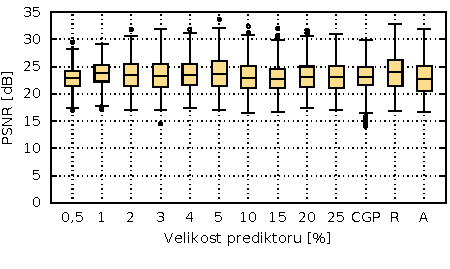
\includegraphics[width=0.475\textwidth]{fig/plot/compare/saltpepper20-100kg-psnrtest.pdf}
    \hskip0.5cm
    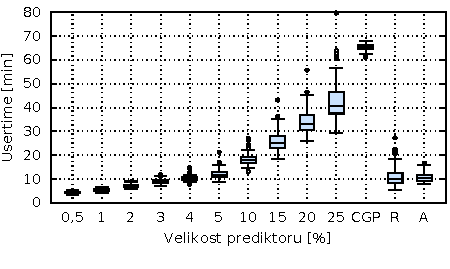
\includegraphics[width=0.475\textwidth]{fig/plot/compare/saltpepper20-100kg-usertime.pdf}
    \caption{20\% šum typu sůl a pepř}
\end{figure}

\begin{figure}[H]
    \centering
    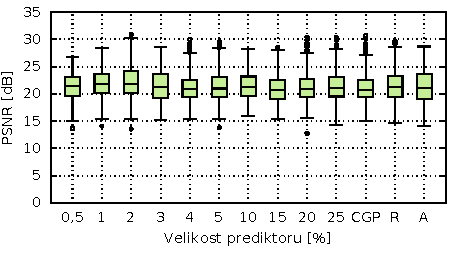
\includegraphics[width=0.475\textwidth]{fig/plot/compare/saltpepper25-100kg-psnrtest.pdf}
    \hskip0.5cm
    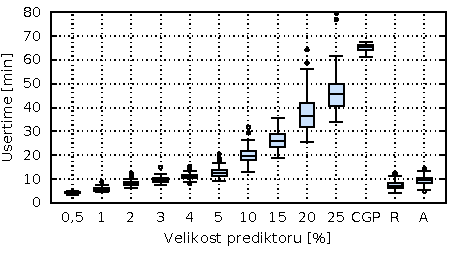
\includegraphics[width=0.475\textwidth]{fig/plot/compare/saltpepper25-100kg-usertime.pdf}
    \caption{25\% šum typu sůl a pepř}
\end{figure}

\begin{figure}[H]
    \centering
    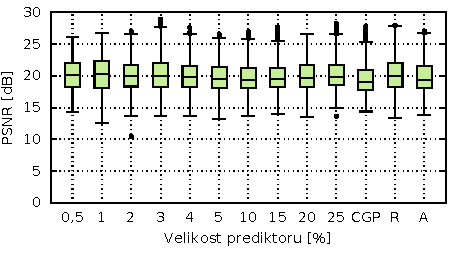
\includegraphics[width=0.475\textwidth]{fig/plot/compare/saltpepper30-100kg-psnrtest.pdf}
    \hskip0.5cm
    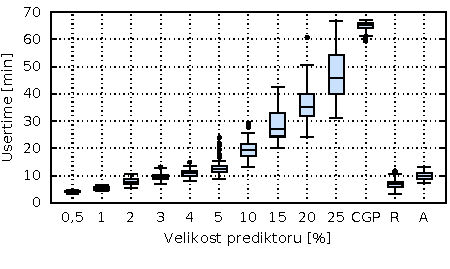
\includegraphics[width=0.475\textwidth]{fig/plot/compare/saltpepper30-100kg-usertime.pdf}
    \caption{30\% šum typu sůl a pepř}
\end{figure}

%\clearpage

\begin{figure}[H]
    \centering
    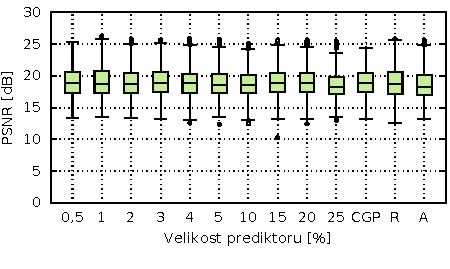
\includegraphics[width=0.475\textwidth]{fig/plot/compare/saltpepper35-100kg-psnrtest.pdf}
    \hskip0.5cm
    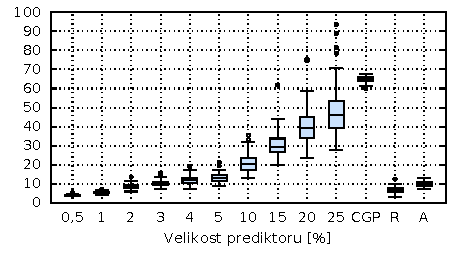
\includegraphics[width=0.475\textwidth]{fig/plot/compare/saltpepper35-100kg-usertime.pdf}
    \caption{35\% šum typu sůl a pepř}
\end{figure}

\begin{figure}[H]
    \centering
    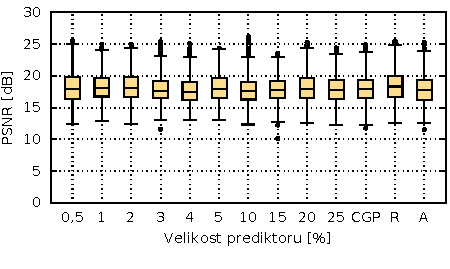
\includegraphics[width=0.475\textwidth]{fig/plot/compare/saltpepper40-100kg-psnrtest.pdf}
    \hskip0.5cm
    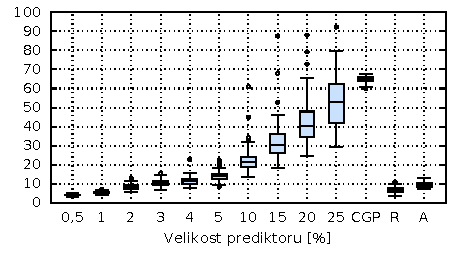
\includegraphics[width=0.475\textwidth]{fig/plot/compare/saltpepper40-100kg-usertime.pdf}
    \caption{40\% šum typu sůl a pepř}
\end{figure}

\begin{figure}[H]
    \centering
    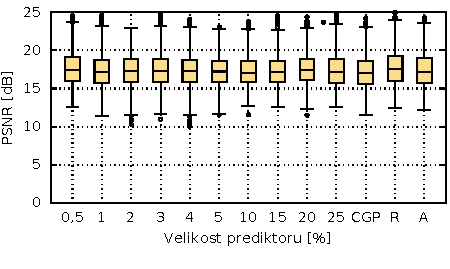
\includegraphics[width=0.475\textwidth]{fig/plot/compare/saltpepper45-100kg-psnrtest.pdf}
    \hskip0.5cm
    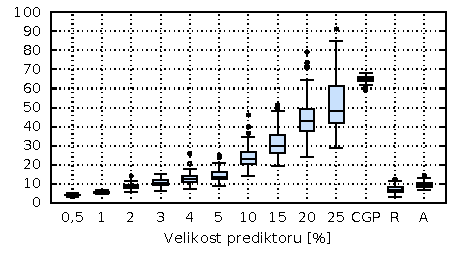
\includegraphics[width=0.475\textwidth]{fig/plot/compare/saltpepper45-100kg-usertime.pdf}
    \caption{45\% šum typu sůl a pepř}
\end{figure}

\begin{figure}[H]
    \centering
    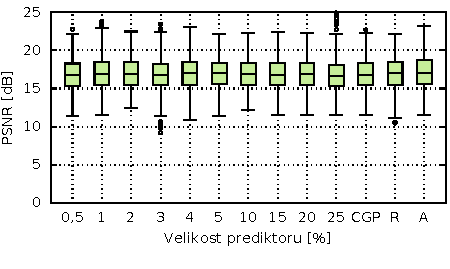
\includegraphics[width=0.475\textwidth]{fig/plot/compare/saltpepper50-100kg-psnrtest.pdf}
    \hskip0.5cm
    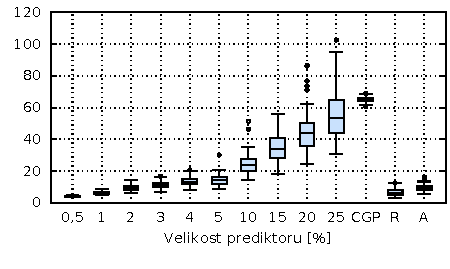
\includegraphics[width=0.475\textwidth]{fig/plot/compare/saltpepper50-100kg-usertime.pdf}
    \caption{50\% šum typu sůl a pepř}
\end{figure}

%\clearpage

\begin{figure}[H]
    \centering
    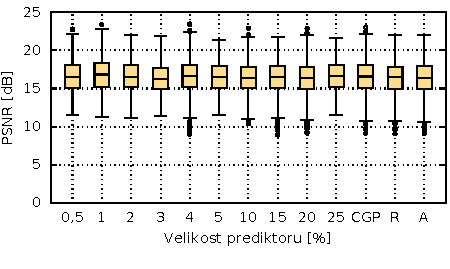
\includegraphics[width=0.475\textwidth]{fig/plot/compare/saltpepper55-100kg-psnrtest.pdf}
    \hskip0.5cm
    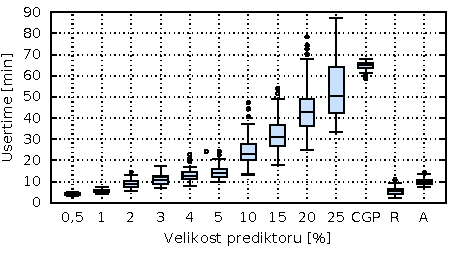
\includegraphics[width=0.475\textwidth]{fig/plot/compare/saltpepper55-100kg-usertime.pdf}
    \caption{55\% šum typu sůl a pepř}
\end{figure}

\begin{figure}[H]
    \centering
    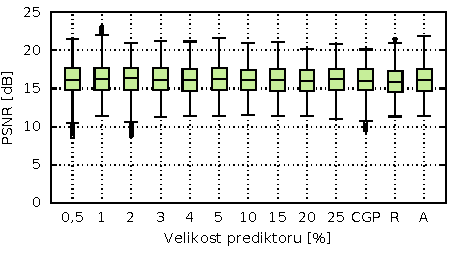
\includegraphics[width=0.475\textwidth]{fig/plot/compare/saltpepper60-100kg-psnrtest.pdf}
    \hskip0.5cm
    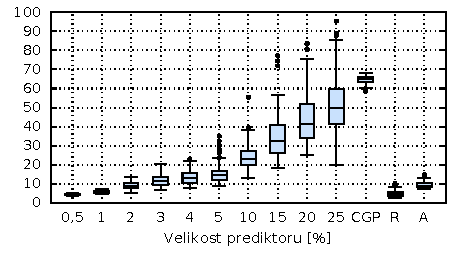
\includegraphics[width=0.475\textwidth]{fig/plot/compare/saltpepper60-100kg-usertime.pdf}
    \caption{60\% šum typu sůl a pepř}
\end{figure}

\begin{figure}[H]
    \centering
    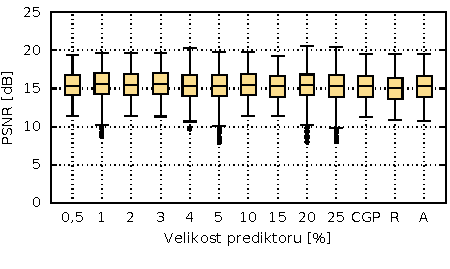
\includegraphics[width=0.475\textwidth]{fig/plot/compare/saltpepper70-100kg-psnrtest.pdf}
    \hskip0.5cm
    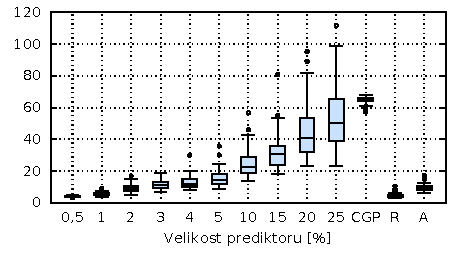
\includegraphics[width=0.475\textwidth]{fig/plot/compare/saltpepper70-100kg-usertime.pdf}
    \caption{70\% šum typu sůl a pepř}
\end{figure}

\begin{figure}[H]
    \centering
    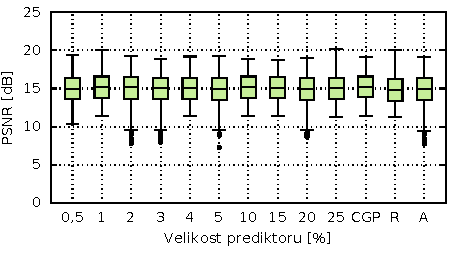
\includegraphics[width=0.475\textwidth]{fig/plot/compare/saltpepper75-100kg-psnrtest.pdf}
    \hskip0.5cm
    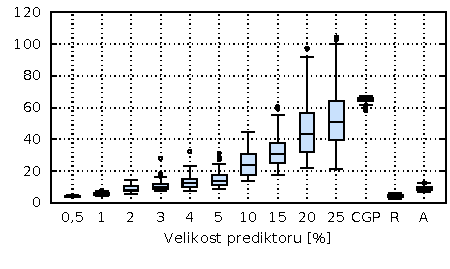
\includegraphics[width=0.475\textwidth]{fig/plot/compare/saltpepper75-100kg-usertime.pdf}
    \caption{75\% šum typu sůl a pepř}
\end{figure}

%\clearpage

\begin{figure}[H]
    \centering
    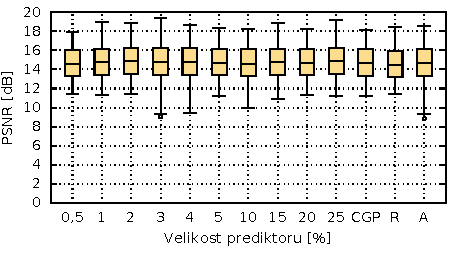
\includegraphics[width=0.475\textwidth]{fig/plot/compare/saltpepper80-100kg-psnrtest.pdf}
    \hskip0.5cm
    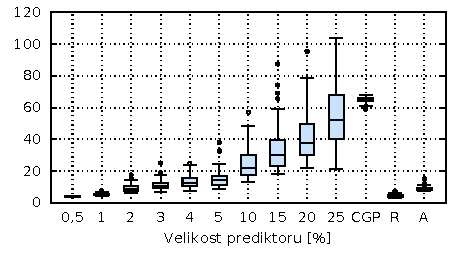
\includegraphics[width=0.475\textwidth]{fig/plot/compare/saltpepper80-100kg-usertime.pdf}
    \caption{80\% šum typu sůl a pepř}
\end{figure}


%%%%%%%%%%%%%%%%%%%%%


\section{Výstřelový šum}


\begin{figure}[H]
    \centering
    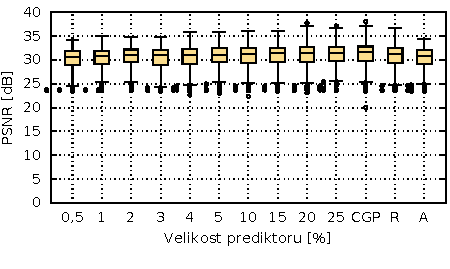
\includegraphics[width=0.475\textwidth]{fig/plot/compare/impulse5-100kg-psnrtest.pdf}
    \hskip0.5cm
    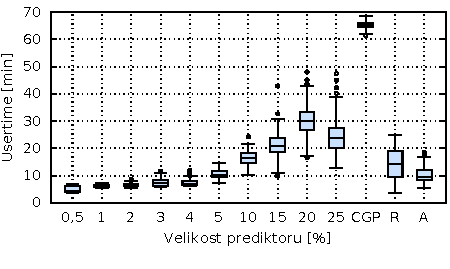
\includegraphics[width=0.475\textwidth]{fig/plot/compare/impulse5-100kg-usertime.pdf}
    \caption{5\% výstřelový (náhodný) šum}
\end{figure}

\begin{figure}[H]
    \centering
    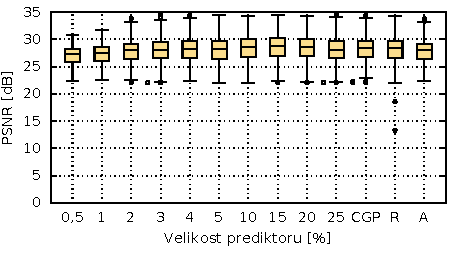
\includegraphics[width=0.475\textwidth]{fig/plot/compare/impulse10-100kg-psnrtest.pdf}
    \hskip0.5cm
    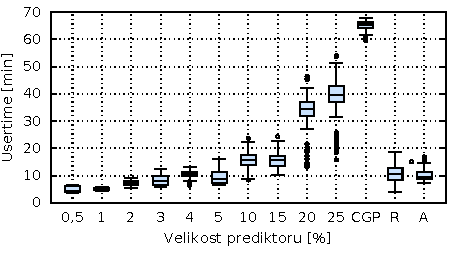
\includegraphics[width=0.475\textwidth]{fig/plot/compare/impulse10-100kg-usertime.pdf}
    \caption{10\% výstřelový (náhodný) šum}
\end{figure}

\begin{figure}[H]
    \centering
    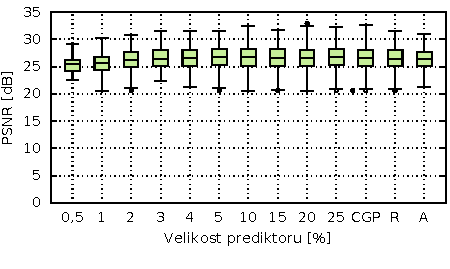
\includegraphics[width=0.475\textwidth]{fig/plot/compare/impulse15-100kg-psnrtest.pdf}
    \hskip0.5cm
    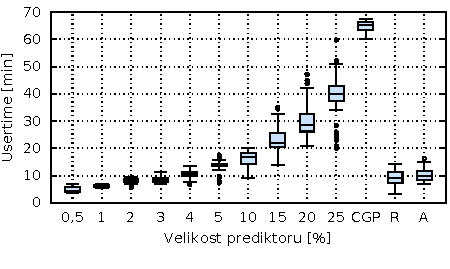
\includegraphics[width=0.475\textwidth]{fig/plot/compare/impulse15-100kg-usertime.pdf}
    \caption{15\% výstřelový (náhodný) šum}
\end{figure}

%\clearpage

\begin{figure}[H]
    \centering
    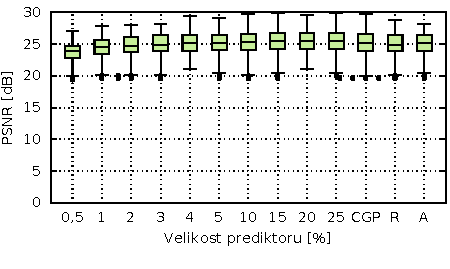
\includegraphics[width=0.475\textwidth]{fig/plot/compare/impulse20-100kg-psnrtest.pdf}
    \hskip0.5cm
    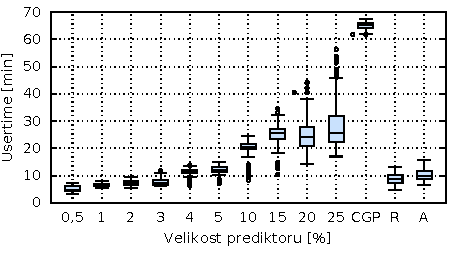
\includegraphics[width=0.475\textwidth]{fig/plot/compare/impulse20-100kg-usertime.pdf}
    \caption{20\% výstřelový (náhodný) šum}
\end{figure}

\begin{figure}[H]
    \centering
    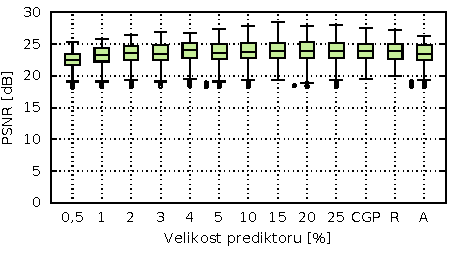
\includegraphics[width=0.475\textwidth]{fig/plot/compare/impulse25-100kg-psnrtest.pdf}
    \hskip0.5cm
    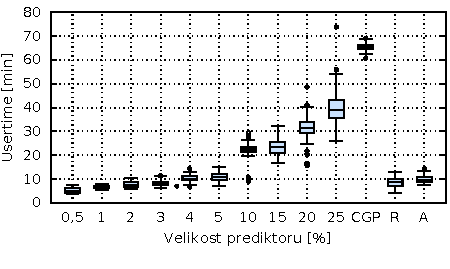
\includegraphics[width=0.475\textwidth]{fig/plot/compare/impulse25-100kg-usertime.pdf}
    \caption{25\% výstřelový (náhodný) šum}
\end{figure}

\begin{figure}[H]
    \centering
    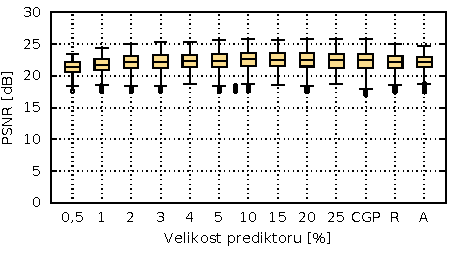
\includegraphics[width=0.475\textwidth]{fig/plot/compare/impulse30-100kg-psnrtest.pdf}
    \hskip0.5cm
    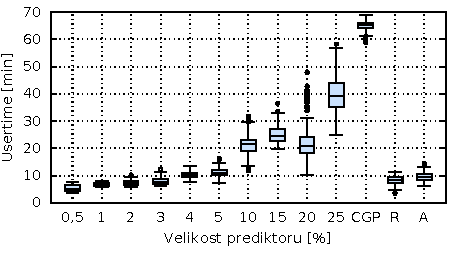
\includegraphics[width=0.475\textwidth]{fig/plot/compare/impulse30-100kg-usertime.pdf}
    \caption{30\% výstřelový (náhodný) šum}
\end{figure}

\begin{figure}[H]
    \centering
    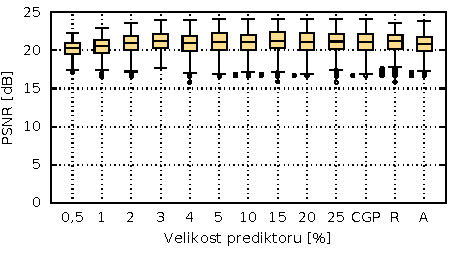
\includegraphics[width=0.475\textwidth]{fig/plot/compare/impulse35-100kg-psnrtest.pdf}
    \hskip0.5cm
    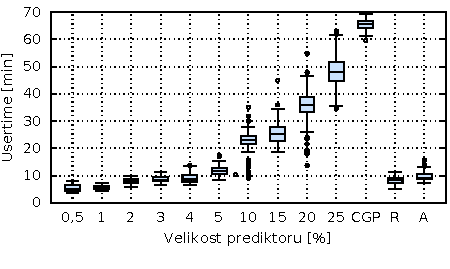
\includegraphics[width=0.475\textwidth]{fig/plot/compare/impulse35-100kg-usertime.pdf}
    \caption{35\% výstřelový (náhodný) šum}
\end{figure}

%\clearpage

\begin{figure}[H]
    \centering
    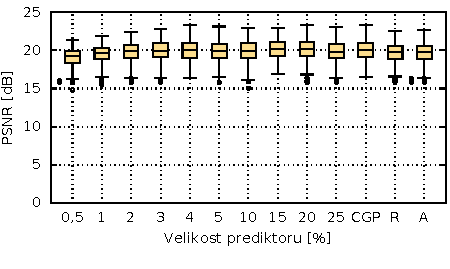
\includegraphics[width=0.475\textwidth]{fig/plot/compare/impulse40-100kg-psnrtest.pdf}
    \hskip0.5cm
    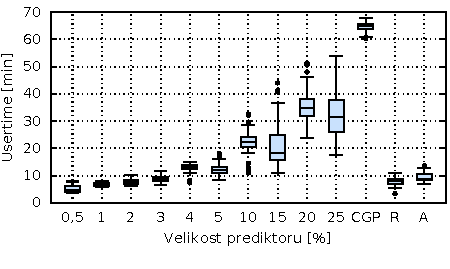
\includegraphics[width=0.475\textwidth]{fig/plot/compare/impulse40-100kg-usertime.pdf}
    \caption{40\% výstřelový (náhodný) šum}
\end{figure}

\begin{figure}[H]
    \centering
    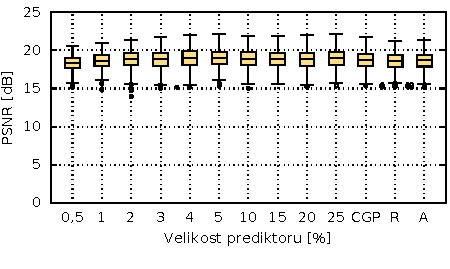
\includegraphics[width=0.475\textwidth]{fig/plot/compare/impulse45-100kg-psnrtest.pdf}
    \hskip0.5cm
    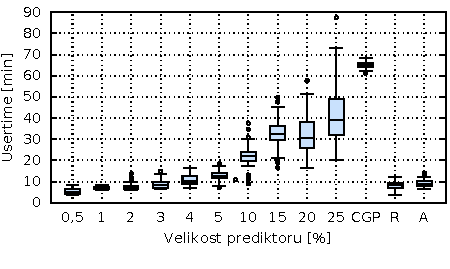
\includegraphics[width=0.475\textwidth]{fig/plot/compare/impulse45-100kg-usertime.pdf}
    \caption{45\% výstřelový (náhodný) šum}
\end{figure}

\begin{figure}[H]
    \centering
    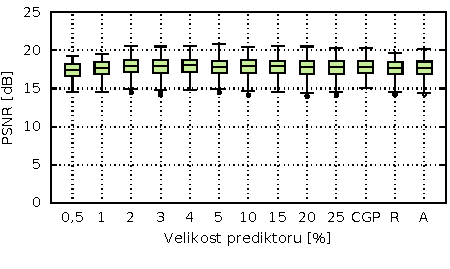
\includegraphics[width=0.475\textwidth]{fig/plot/compare/impulse50-100kg-psnrtest.pdf}
    \hskip0.5cm
    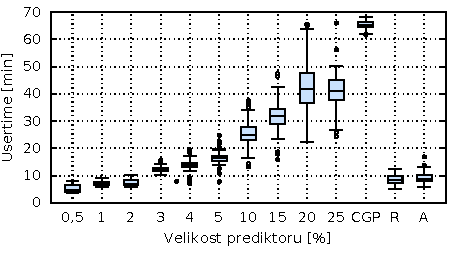
\includegraphics[width=0.475\textwidth]{fig/plot/compare/impulse50-100kg-usertime.pdf}
    \caption{50\% výstřelový (náhodný) šum}
\end{figure}

\begin{figure}[H]
    \centering
    \includegraphics[width=0.475\textwidth]{fig/plot/compare/impulse55-100kg-psnrtest.pdf}
    \hskip0.5cm
    \includegraphics[width=0.475\textwidth]{fig/plot/compare/impulse55-100kg-usertime.pdf}
    \caption{55\% výstřelový (náhodný) šum}
\end{figure}

%\clearpage

\begin{figure}[H]
    \centering
    \includegraphics[width=0.475\textwidth]{fig/plot/compare/impulse60-100kg-psnrtest.pdf}
    \hskip0.5cm
    \includegraphics[width=0.475\textwidth]{fig/plot/compare/impulse60-100kg-usertime.pdf}
    \caption{60\% výstřelový (náhodný) šum}
\end{figure}

\begin{figure}[H]
    \centering
    \includegraphics[width=0.475\textwidth]{fig/plot/compare/impulse70-100kg-psnrtest.pdf}
    \hskip0.5cm
    \includegraphics[width=0.475\textwidth]{fig/plot/compare/impulse70-100kg-usertime.pdf}
    \caption{70\% výstřelový (náhodný) šum}
\end{figure}

\begin{figure}[H]
    \centering
    \includegraphics[width=0.475\textwidth]{fig/plot/compare/impulse75-100kg-psnrtest.pdf}
    \hskip0.5cm
    \includegraphics[width=0.475\textwidth]{fig/plot/compare/impulse75-100kg-usertime.pdf}
    \caption{75\% výstřelový (náhodný) šum}
\end{figure}

\begin{figure}[H]
    \centering
    \includegraphics[width=0.475\textwidth]{fig/plot/compare/impulse80-100kg-psnrtest.pdf}
    \hskip0.5cm
    \includegraphics[width=0.475\textwidth]{fig/plot/compare/impulse80-100kg-usertime.pdf}
    \caption{80\% výstřelový (náhodný) šum}
\end{figure}

%\clearpage


%%%%%%%%%%%%%%%%%%


\section{Detektor hran}

\begin{figure}[H]
    \centering
    \includegraphics[width=0.475\textwidth]{fig/plot/compare/sobelsobel1b-100kg-psnr.pdf}
    \hskip0.5cm
    \includegraphics[width=0.475\textwidth]{fig/plot/compare/sobelsobel1b-100kg-usertime.pdf}
    \caption{Detektor hran}
\end{figure}
